
% Opisowy model stanu istniejącego
% Opis wszystkich składników organizacyjnych
% Związek struktury z dziedziną obszaru modelowania, wyznaczenie zakresu odpowiedzialności systemu 	

\paragraph{Grupa Kapitałowa Biosystem} składa się z trzech podmiotów gospodarczych (\emph{BIOSYSTEM S.A.}, \emph{BIOSYSTEM Elektrorecykling Organizacja Odzysku Sprzętu Elektrycznego i Elektronicznego S.A.}, \emph{Zakład Gospodarki Komunalnej Organizacja Odzysku BIOSYSTEM S.A.}. Firma \emph{BIOSYSTEM S.A.} stanowi spółkę nadrzędną.

\begin{figure}[H]
	\centering
	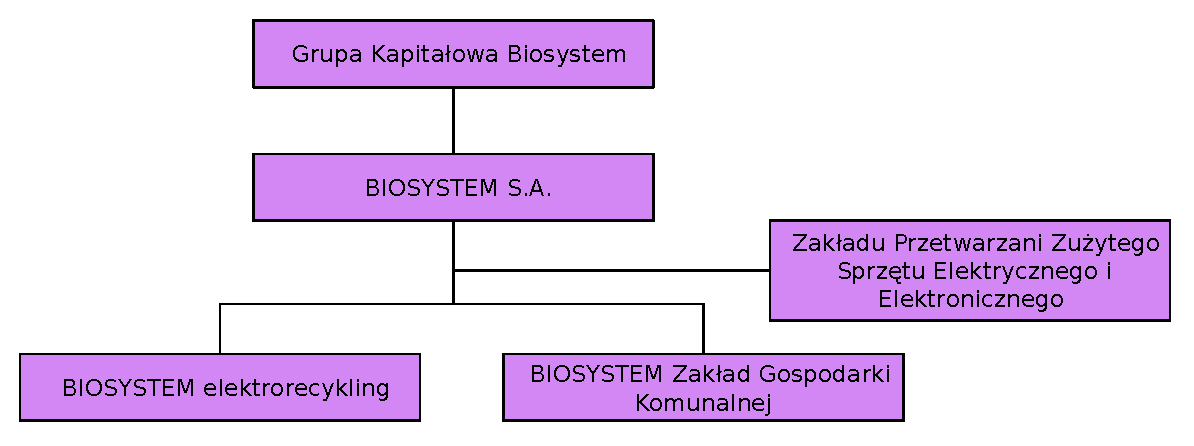
\includegraphics[width=\textwidth]{img/group_chart.eps}
	\caption{Struktura grupy kapitałowej}
\end{figure}

\paragraph{Opis składników organizacyjnych} \ \\
Dwa z tych podmiotów zajmują się sprawozdawczością wobec Urzędów Marszałkowskich zgodnie z ustawą o odpadach.
W ramach działalności współpracują z klientami wprowadzającymi różnego rodzaju materiały do środowiska, które powinny podlegać recyklingowi.
W związku z tym prowadzą działalność dodatkową polegającą na zbieraniu opakowań z papieru, tworzyw sztucznych, szkła, blachy i aluminium oraz sprzętu elektrycznego i elektronicznego.
Spółka BIOSYSTEM S.A. jest również właścicielem \emph{Zakład Przetwarzania Zużytego Sprzętu Elektrycznego i Elektronicznego}, który zajmuje się recyklingiem sprzętu elektrycznego i elektronicznego. 

\paragraph{Odpowiedzialność poszczególnych spółek} \ \\
\begin{enumerate}
	\item \emph{BIOSYSTEM S.A.}: 
		\begin{itemize}
			\item działalność handlowa
			\item nadzór właścicielski nad spółkami zależnymi
		\end{itemize}
	\item \emph{BIOSYSTEM elektrorecykling}: sprawozdawczość w zakresie wprowadzania sprzętu elektrycznego i elektronicznego przez swoich klientów \\
	\item \emph{BIOSYSTEM ZGK}:
		\begin{itemize}
			\item sprawozdawczość w zakresie wprowadzania opakowań i baterii przez swoich klientów
			\item organizacja przetwarzania opakowań przy pomocy firm współpracujących
		\end{itemize}
\end{enumerate}

\paragraph{Wewnętrzna struktura organizacyjna} \ \\

\begin{figure}[H]
    \centering
    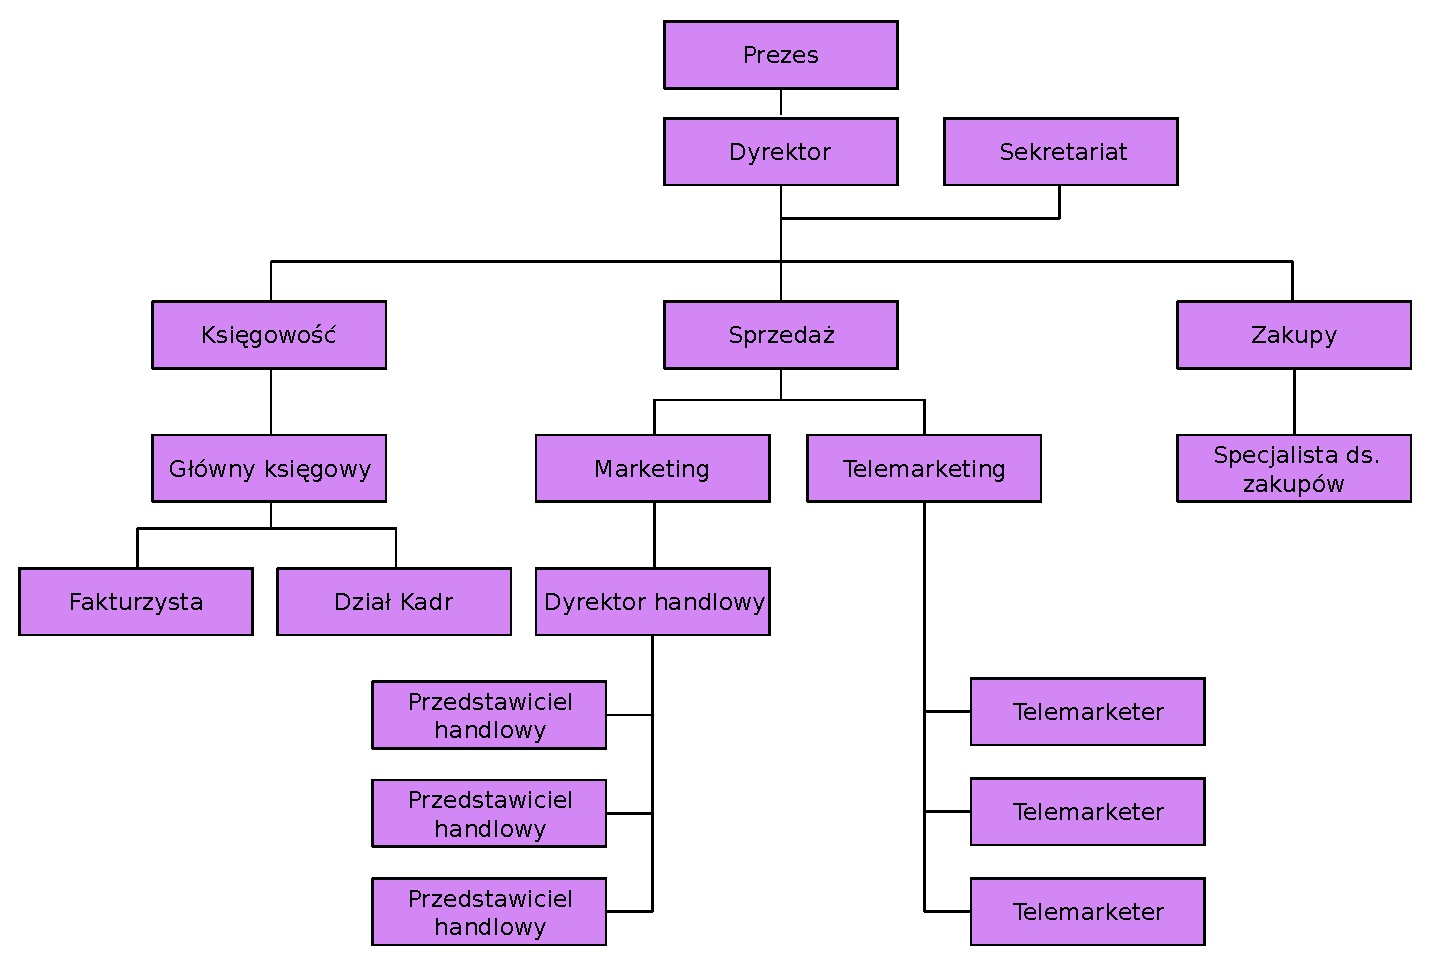
\includegraphics[width=1\textwidth]{img/organization_chart.eps}
    \caption{Struktura organizacyjna spółki}
\end{figure}